\chapter{Integrating the simulator into Kubernetes}

\subsubsection{Problematic}

Batsim is able to run simulations of any distributed system, to study any
event-based scheduler that would implement its message protocol. Kubernetes is
a piece of software where all its component, including the scheduler, revolve
around a central API. Everything is then asynchronous as the API can be
accessed anytime by any component.

The question that arises is, can we adapt Batsim to make it support Kubernetes
schedulers? Is it possible to implement an adaptive layer between a synchronous
event based simulator like Batsim and a scheduler implemented following the
asynchronous paradigms of APIs?

It will follow that in order to do so, we re-implemented an API following
Kubernetes specifications and intercepted the scheduler's time to
synchronize it with the simulation time. This allows us to run lengthy
workloads in seconds using a scheduler otherwise supposed to rely on ``real''
machine time. We first describe some technical concepts about Kubernetes and
Batsim, and then describe how we re-implemented the API, intercepted the time,
and handled the synchronization of the different times between Batsim and the
scheduler.

\section{Batsim concepts}

A Batsim simulation is divided into two processes: Batsim itself and the
decision process (the scheduler). Both process exchange via the ZeroMQ
request-reply
pattern\footnote{\url{http://zguide.zeromq.org/page:all\#Ask-and-Ye-Shall-Receive}}.
As a consequence, the scheduler must be event based and implement Batsim's
Protocol.

\begin{figure}[H]
	\centering
	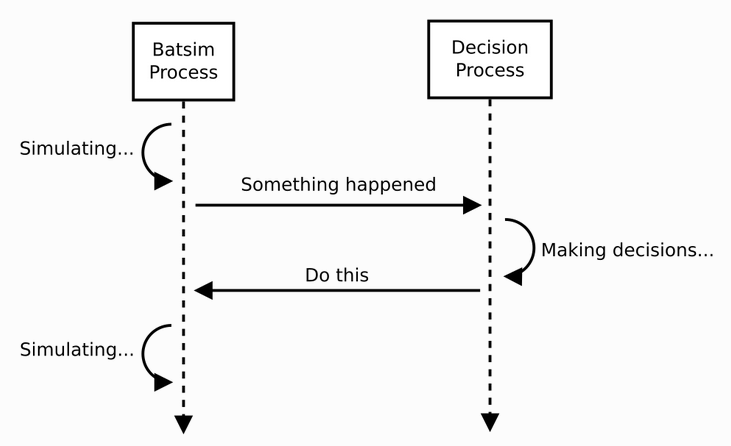
\includegraphics[scale=0.5]{imgs/batsim-sequence-diag.png}
	\captionsource{Exchanges between Batsim and the scheduler}{https://batsim.readthedocs.io/en/latest/protocol.html}
	\label{fig:bati-seq-diag}
\end{figure}

Batsim messaging interface is based on its protocol. Each message is composed
of the current simulation time, as well as a list of events either from Batsim
to the scheduler, or from the scheduler to Batsim. Figure \ref{fig:batmsg_ex}
depicts a standard message sent from the scheduler to Batsim.

\begin{figure}
\begin{minted}{js}
{
  "now": 1024.24,
  "events": [
    {
      "timestamp": 1000,
      "type": "EXECUTE_JOB",
      "data": {
        "job_id": "workload!job_1234",
        "alloc": "1 2 4-8",
      }
    },
    {
      "timestamp": 1012,
      "type": "EXECUTE_JOB",
      "data": {
        "job_id": "workload!job_1235",
        "alloc": "12-100",
      }
    }
  ]
}
\end{minted}
\caption{Example of a Batsim message}
\label{fig:batmsg_ex}
\end{figure}

Batkube's features being very basic because we focused on building a working
proof of concept rather than a fully fledged Kubernetes simulator, we only
consider a subset of these messages that we briefly present here. More
information on Batsim's protocol is available on Batsim
documentation\footnote{https://batsim.readthedocs.io/en/latest/protocol.html}

\subsubsection{From Batsim to the scheduler}

\paragraph{SIMULATION\_BEGINS}
contains mostly information about the available resources in the cluster, with
Batsim's configuration.

\paragraph{SIMULATION\_ENDS}
is sent at the very end of the simulation: all jobs have finished, and no more
jobs are left in the queues. Batsim exits this message.

\paragraph{JOB\_SUBMITTED}
notifies the scheduler that a new job has been submitted. It contains
information about the job type, id and specifications. We only consider jobs of
type \textit{delay} to simplify the models. Delay jobs specifications boil down
to the delay length, to which we add resource requests.

\paragraph{JOB\_COMPLETED}
notifies the scheduler that a job has ended, specifying the reason for it. We
only consider situations where all jobs complete correctly. Their state is then
always COMPLETED\_SUCCESSFULLY in our case.

\paragraph{REQUESTED\_CALL}
is an awnser to a CALL\_ME\_LATER event sent by the scheduler.

\subsubsection{From the scheduler to Batsim}

\paragraph{CALL\_ME\_LATER}
is an incentive from the scheduler for Batsim to wake up at a certain
timestamp. When the timestamp is reached in the simulation, Batsim will send a
REQUESTED\_CALL to the scheduler. In our case, this particular exchange will
serve as the base for time synchronisation between the scheduler and Batsim.

\paragraph{EXECUTE\_JOB}
is sent when the scheduler has made a decision. It contains the id of the job
at stake and the id of the resources it has been scheduled to.

\subsubsection{Bidirectional}

\paragraph{NOTIFY}
is used to send some information to the other peer. In our case, we use the
NOTIFY containing no\_more\_static\_job\_to\_submit to determine if the
simulation has ended: knowing that there are no more jobs susceptible to be
scheduled allow us to fast forward to the end of the simulation, thus saving
execution time.\\

Batsim's output takes the form of a csv file containg information about the
jobs executions. Mainly we take interest in their submission time, execution
time and waiting time. Again, a detailed list of Batsim outputs can be found on
the
documentation\footnote{https://batsim.readthedocs.io/en/latest/output-jobs.html}.
During our experimentations with Batkube we interest ourselves in two metrics
that can be computed from this output:
\begin{itemize}
	\item The \textit{makespan}, which is the total length of the
		simulation. It is defined as the timestamp at which the last
		job finishes executing, minus the origin (in this case, zero).
	\item The \textit{mean\_waiting\_time}, which is the mean time the jobs
		spent waiting for a scheduling decision. The waiting time is
		defined by the duration between the submission time and the
		starting time (here the starting time is equivalent to the time
		at which the job was scheduled. We will see later that these
		two times do not correspond in Kubernetes.)
\end{itemize}

\section{Kubernetes concepts}

Kubernetes is a large ecosystem that we can not possibly describe or study in
its entirety in the short amount of time that was allocated to this project.
Instead, let us focus on some details about scheduling in Kubernetes and how it
differs from the Batsim approach.

\begin{figure}[h]
	\centering
	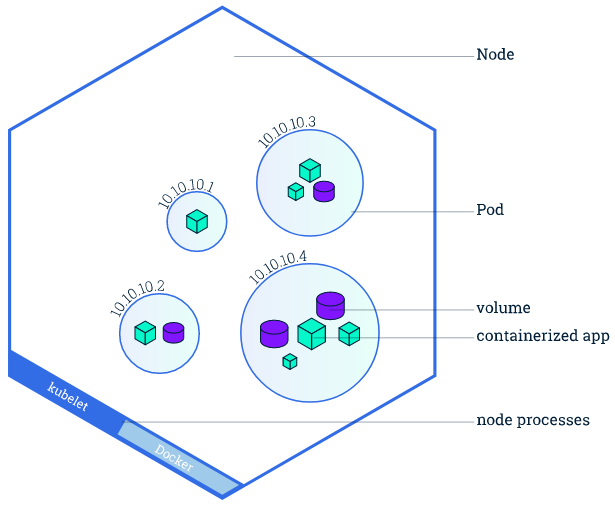
\includegraphics[scale=0.5]{./imgs/node-overview.png}
	\captionsource{Node overview}{https://kubernetes.io/docs/tutorials/kubernetes-basics/explore/explore-intro/}
	\label{fig:node-overview}
\end{figure}

The basic processing unit of Kubernetes is called a \textbf{pod} which is
composed of one or several containers and volumes\footnote{Because of their
	transient nature, containers can not store data on their own. A volume
	is some storage space on the host machine that can be linked to
containers, in order for them to read and write persistent information.}. The
type of application they contain vary depending on the context: in a web
platform context a pod most often hosts a service or micro-service that must be
available at all times, in opposition to a batch processing context where it
runs an application that is to be executed in a finite amount of time.  Pods
are bundled together in \textbf{nodes} (figure \ref{fig:node-overview}) which
are either physical or virtual machines. They represent another barrier to pass
through to access the outside world which bundles pods under the same network
to facilitate communication between them, and enables the use of proxies to
access the underlying services. A set of nodes is called a \textbf{cluster}
which is the highest abstraction layer in Kubernetes.

Nodes take the idea of containerisation further than plain containers by
encapsulating the already encapsulated services.  Each node runs at least one
pod, the \textbf{kubelet}, which is a process responsible for communicating
with the rest of Kubernetes. More precisely, the kubelet communicates with the
\textbf{kube-api-server} which is responsible for the whole cluster.  This API
server, as well as the other components of the \textbf{Control Plane} (figure
\ref{fig:kube-components}), can be run on any machine but for simplicity they
are set up on the same machine at start up. This machine is often called the
\textbf{master} node and typically does not run any other container.

As stated before Kubernetes revolves around its API server which is its central
component. All operations between components go through this REST API. These
operations take various forms like user interactions through the commande line
interface \textbf{kubectl}, scheduling operations or management of cluster data
on \textbf{etcd}. We then decided to re-build the API in order to simulate any
cluster to -- almost -- any Kubernetes scheduler.

\begin{figure}[h]
	\centering
	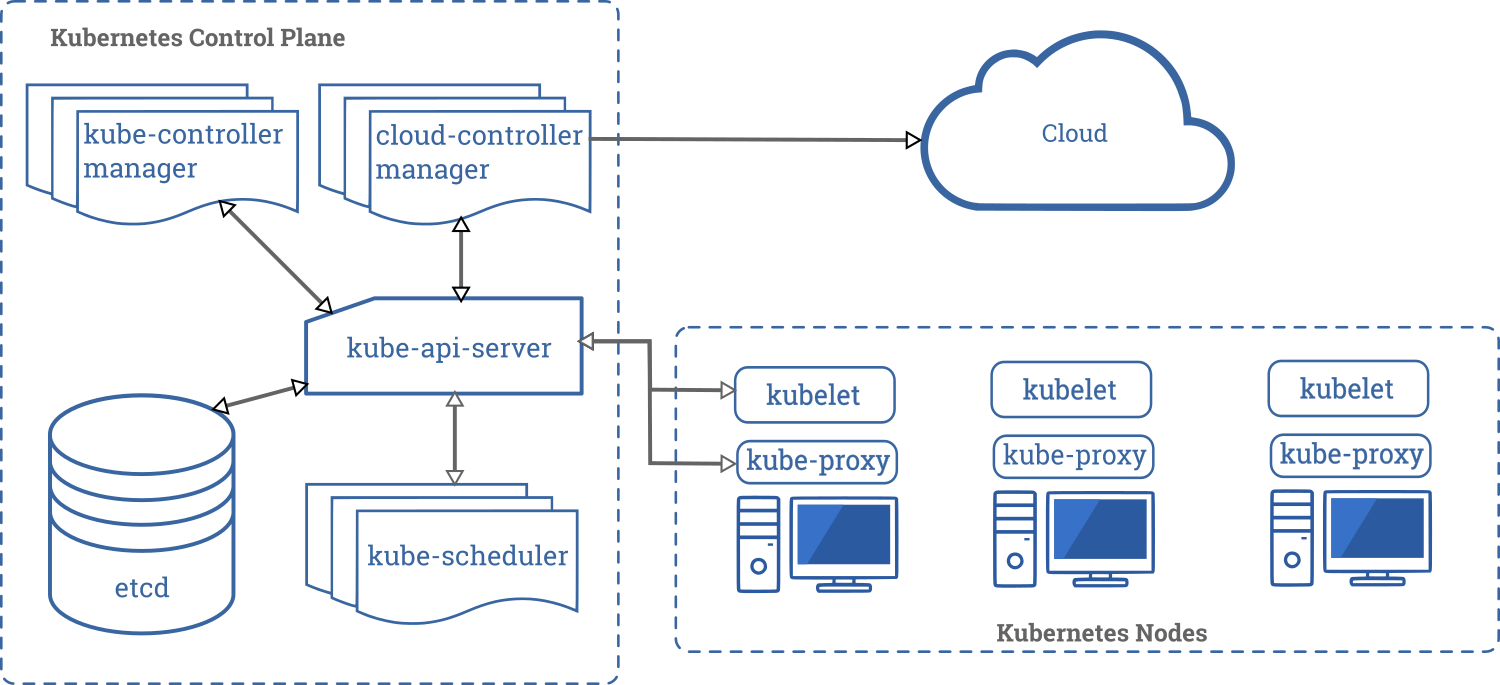
\includegraphics[width=\textwidth]{./imgs/components-of-kubernetes.png}
	\captionsource{Components of Kubernetes}{https://kubernetes.io/docs/concepts/overview/components/}
	\label{fig:kube-components}
\end{figure}

%\subsection{HPC and Kubernetes}
%The difference between HPC and Cloud Native computing lies in the workloads
%they are intended to tackle.  Kubernetes was designed for Cloud Native
%applications. Services or micro services are run in containers and are expected
%to be available at all times : they are replicated as many times as the user
%desires and restarted whenever a failure occurs. High availability is at the
%core of Kubernetes container management.  On the other hand, depending on
%scheduling policies, HPC is focused on user wait time, maximizing resource
%usage, optimizing energy costs... For instance, in case of failure, it is
%sometimes not sufficient to restart the single job that failed : the entire
%submission must be re-run if it is part of several jobs computed in parallel.
%
%Kubernetes is now the standard for AI and Machine Learning as shown by the many
%efforts at making this coupling an efficient
%environment\cite{lee2017design}\cite{233001}\cite{10.1145/3154842.3154845},
%which brought an increasing interest for container driven HPC aswell and
%Kubernetes for HPC in particular. Batch schedulers such as
%kube-batch\footnote{\url{https://github.com/kubernetes-sigs/kube-batch}} have
%been implemented for kube, and numerous HPC applications like
%slurm\footnote{\url{https://slurm.schedmd.com/containers.html}} now support containers as well.
%
%Indeed, containers have many advantages that HPC users can benefit from. Here
%are some notable ones:
%\begin{itemize}
%	\item First off, research has shown that Kuberenetes offer similar
%		performance to more standard bare metal HPC\cite{8950981}.
%	\item Users will get the same environment everywhere making up for a
%		uniform and standardized workplace.
%	\item Portability : users could seamlessly hop from one infrastructure
%		to another based on their needs and criteria like price,
%		performance, and capabilities rather than compatibility.
%	\item Encapsulation : HPC applications often rely on complex
%		dependencies that can be easily concealed into containers.
%\end{itemize}
%\begin{figure}[h]
%	\centering
%	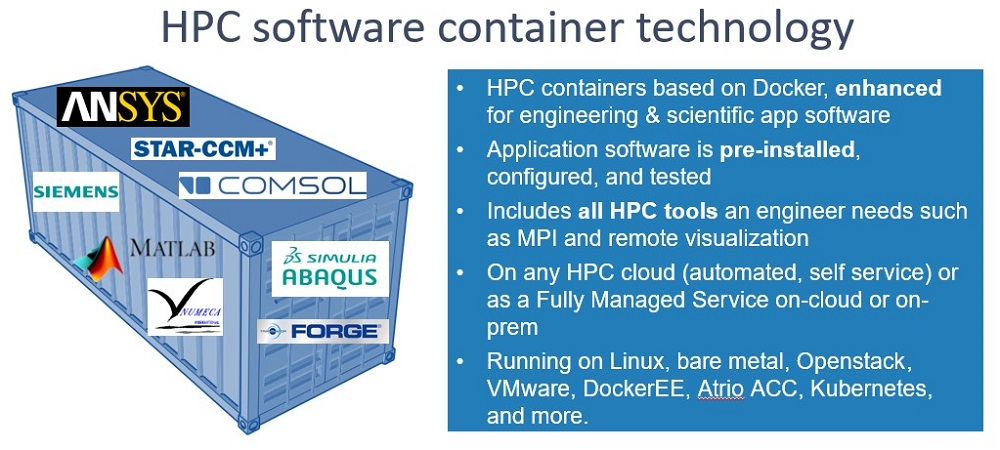
\includegraphics[scale=0.5]{./imgs/hpc-container.jpg}
%	\captionsource{The container technology for HPC}{https://www.hpcwire.com/2019/09/19/kubernetes-containers-and-hpc/}
%	\label{fig:hpc-container}
%\end{figure}
%
%Despite all those advantages, Kubernetes is not ready yet to be used in proper
%HPC environment because it lacks vital components like a proper batch job
%queuing system, and support for MPI applications. It cannot yet compete against
%the very well established HPC ecosystem, but that time may come soon as
%containers are becoming more and more integrated in modern infrastructures.

\section{Re-building the API}

TODO: Explain hy this is the best approach we could find and how we did it.

\section{Translation and resource management}

TODO: maybe move this section under the last section. This is a minor problem
and was really not too dificult in our case. Maybe explain why we did not
translate batsim jobs to kubernetes jobs but rather directly to pods.

Explain how dirty the resource management system is (non thread safe, stored in
memory, little hacks for the resource version) and briefly write on how it
induces problems on the scheduling (overlap of jobs on the same resource where
there is no room for them) (we talk about this in the evaluation part).

\section{Time interception}

TODO: explain how channels work briefly, to understand the algorithms.

\SetKwInput{KwInput}{Input}
\SetKwInput{KwOutput}{Output}


\begin{algorithm}[H]
\DontPrintSemicolon
\KwInput{req: request channel, res: result channel map}
\While{Batkube is not ready} {
	wait\;
}
requests = []request\;
\While{req is not empty} {
	m = $<$- req \tcc{Non blocking receive}
	requests = append(requests, m)\;
}
sendToBatkube(requests) \tcc{Only requests with duration > 0 are actually sent. Batkube will always anwser.}
now = responseFromBatkube()\;
\For{m in range requests} {
	res[m.id] $<$-now \tcc{The caller continues execution upon reception}
}

	
\caption{Requester loop}
\label{alg:reqLoop}
\end{algorithm}


\begin{algorithm}[H]
\DontPrintSemicolon
\KwResult{Current simulation time}
\KwInput{d: timer duration, req: request channel, res: response channel map}
\KwOutput{now : simulation time}

\If{requester loop is not running}{
	go runRequesterLoop() \tcc{There can only be one loop runing at a time}
}
id = newUUID()\;
m = newRequestMessage(d, id) \tcc{Requests are identified using uuids}
resChannel = newChannel()\;
res[id] = resChannel \tcc{A channel is associated with each request}
req $<$- m \tcc{The code blocks here until request is handled}
now = $<$-resChannel \tcc{The code blocks here until response is sent by the requester loop}
return now\;
\caption{Time request (time.now())}
\label{alg:now}
\end{algorithm}


\section{Time synchronization}

\begin{figure}[H]
	\centering
	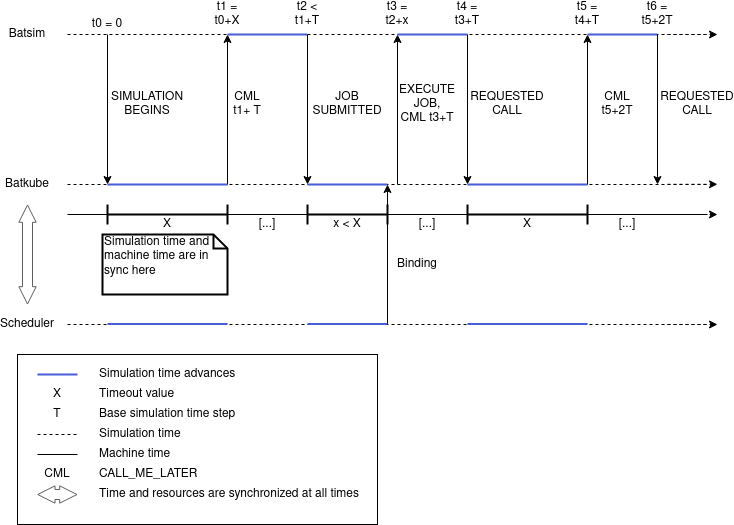
\includegraphics[width=\textwidth]{imgs/lignes_de_temps.png}
	\caption{Time sync between the three components. The broker has to take
	into account both machine time and simulation time.}
	\label{fig:time_sync}
\end{figure}



